\documentclass[bachelor, och, coursework]{SCWorks}
% параметр - тип обучения - одно из значений:
%    spec     - специальность
%    bachelor - бакалавриат (по умолчанию)
%    master   - магистратура
% параметр - форма обучения - одно из значений:
%    och   - очное (по умолчанию)
%    zaoch - заочное
% параметр - тип работы - одно из значений:
%    referat    - реферат
%    coursework - курсовая работа (по умолчанию)
%    diploma    - дипломная работа
%    pract      - отчет по практике
% параметр - включение шрифта
%    times    - включение шрифта Times New Roman (если установлен)
%               по умолчанию выключен
\usepackage{subfigure}
\usepackage{tikz,pgfplots}
\pgfplotsset{compat=1.5}
\usepackage{float}

%\usepackage{titlesec}
\setcounter{secnumdepth}{4}
%\titleformat{\paragraph}
%{\normalfont\normalsize}{\theparagraph}{1em}{}
%\titlespacing*{\paragraph}
%{35.5pt}{3.25ex plus 1ex minus .2ex}{1.5ex plus .2ex}

\titleformat{\paragraph}[block]
{\hspace{1.25cm}\normalfont}
{\theparagraph}{1ex}{}
\titlespacing{\paragraph}
{0cm}{2ex plus 1ex minus .2ex}{.4ex plus.2ex}

% --------------------------------------------------------------------------%


\usepackage[T2A]{fontenc}
\usepackage[utf8]{inputenc}
\usepackage{graphicx}
\graphicspath{ {./images/} }
\usepackage{tempora}

\usepackage[sort,compress]{cite}
\usepackage{amsmath}
\usepackage{amssymb}
\usepackage{amsthm}
\usepackage{fancyvrb}
\usepackage{listings}
\usepackage{listingsutf8}
\usepackage{longtable}
\usepackage{array}
\usepackage[english,russian]{babel}

% \usepackage[colorlinks=true]{hyperref}
\usepackage{url}

\usepackage{underscore}
\usepackage{setspace}
\usepackage{indentfirst} 
\usepackage{mathtools}
\usepackage{amsfonts}
\usepackage{enumitem}
\usepackage{tikz}
\usepackage{minted}

\newcommand{\eqdef}{\stackrel {\rm def}{=}}
\newcommand{\specialcell}[2][c]{%
\begin{tabular}[#1]{@{}c@{}}#2\end{tabular}}

\renewcommand\theFancyVerbLine{\small\arabic{FancyVerbLine}}

\newtheorem{lem}{Лемма}

\begin{document}

% Кафедра (в родительном падеже)
\chair{теоретических основ компьютерной безопасности и криптографии}

% Тема работы
\title{Машинное обучение и трейдинг}

% Курс
\course{3}

% Группа
\group{331}


\department{факультета КНиИТ}

\napravlenie{10.05.01 "--- Компьютерная безопасность}

\author{Никитина Арсения Владимировича}

% Заведующий кафедрой
\chtitle{} % степень, звание
\chname{Абросимов М. Б.}

%Научный руководитель (для реферата преподаватель проверяющий работу)
\satitle{доцент} %должность, степень, звание
\saname{Абросимов М. Б.}

\date{2022}

\maketitle

% Включение нумерации рисунков, формул и таблиц по разделам
% (по умолчанию - нумерация сквозная)
% (допускается оба вида нумерации)
% \secNumbering

%-------------------------------------------------------------------------------------------

\tableofcontents

\intro
    В последнее время анализ курсов акций является немаловажной проблемой. Так
    различают фундаментальный анализ, основанный на финансовой и производственной
    деятельности компаний, а также на общей экономической обстановке выбранной 
    сферы. Также определен технический анализ, который основан на прогнозировании 
    изменения курсов в зависимости от закономерностей изменений цен в прошлом в 
    аналогичных обстоятельствах.

    Таким образом, в данной работе будет рассмотрена концепция технического
    анализа, его основные методы, инструменты, а также будет разработан
    детерминированный алгоритм нахождения технических фигур технического анализа.
    
    Более 150 лет торговые залы Чикагской фондовой биржи были местом проведения 
    торговых сделок покупки и продажи.

    Вплоть до 1997 года более 10 тысяч людей торговали в общих залах 
    Чикагских бирж (в так называемых "биржевых ямах"). Позднее, в том же году 
    появилась торговля с помощью компьютеров. Сейчас только около 10\% трейдеров 
    продолжают торговать в биржевых залах (остальные 90\% торгуют с компьютеров).

    Несложно догадаться, что большинство трейдеров, использующих в качестве
    основного инструмента заработка компьютер, пользуются также различными
    вспомогательными средствами, обеспечивающие им уверенность в своих действиях.

    Итак, одним из средств, помогающих выполнять анализ поведения котировок
    акций, является технический анализ и, в частности, нахождение и анализ
    технических фигур.

\defabbr
    Перед анализом теоретической составляющей машинного обучения и технического
    анализа в трейдинге, стоит ввести ряд терминов и определений,
    являющихся основой для понимания работы алгоритмов поиска технических фигур,
    а также для определения основных составляющих трейдинга.

    \textit{Трейдинг} "--- покупка и продажа акций компаний с целью заработка на 
    ежедневном демпинге цен. Трейдеры внимательно следят за краткосрочными 
    колебаниями цен на эти акции, а затем пытаются купить подешевле и продать 
    подороже. Этот краткосрочный подход отличает биржевых трейдеров от 
    традиционных инвесторов фондового рынка, которые склонны работать в 
    долгосрочной перспективе.

    \textit{Технический анализ} "--- это торговая дисциплина, используемая для 
    оценки инвестиций и выявления торговых возможностей путем анализа статистических 
    тенденций, полученных в результате торговой деятельности, таких как движение 
    цены и объем. В отличие от фундаментального анализа, который пытается оценить 
    стоимость ценной бумаги на основе результатов бизнеса, таких как продажи и 
    прибыль, технический анализ фокусируется на изучении цены и объема.

    \textit{Фигура технического анализа} "--- определенная закономерность подряд 
    идущих значений курса акции, которая отображаются на графике и позволяют 
    трейдеру получать определенные сигналы о том, как стоимость актива будет 
    строиться в будущем.

    \textit{Волатильность} "--- финансовый показатель, отражающий то, как сильно 
    меняется цена на актив или товар за короткий промежуток времени.[1]

    \textit{Искусственный интеллект} (англ. Artificial Intelligence) "---
    технология создания алгоритмов, лежащих в основе проектирования
    интеллектуальных машин и программ, способных имитировать деятельность
    человека.

    \textit{Нейронная сеть (нейросеть)} (англ. Neural Network) "---
    математическая модель, чаще всего имеющая программную интерпретацию, сутью
    которой является реализация деятельности, похожей на деятельность
    биологических нейронных сетей. Нейронная сеть используется при создании
    какого-либо из алгоритмов искусственного интеллекта и состоит из
    совокупности нейронов, соединенных между собой связями. 

    \textit{Признак} (англ. Feature) "--- каждый отдельный элемент информации,
    включаемый в представление о каком-либо анализируемом объекте.

    \textit{Машинное обучение} (англ. Machine Learning) "--- область науки об
    искусственном интеллекте, которая изучает способы создания алгоритмов,
    которые могут обучаться (развиваться).


\section{Теоретическая часть}

    \subsection{Временной ряд}

        \textit{Временной ряд} — это определенные данные, собранные в разные 
        моменты времени, графиком которого является значение времени по оси абсцисс
        и значение наблюдаемой величины в текущий момент времени по оси ординат. [1]

        Временной ряд может иметь детерминированный компонент в определенный момент
        времени, тогда говорят, что данные временного ряда имеют временной тренд.
    
        Временные тренды в данных временных рядов также имеют значение для тестирования 
        и моделирования. Надежность модели временных рядов зависит от правильного 
        определения и учета временных тенденций.
    
        Определить, наличие временного тренда на графике можно с помощью проведения
        возрастающей (убывающей) линии и выявления сосредоточения значений наблюдаемой
        величины в окрестности этой линии.

        \begin{figure}[H]
            \centering
            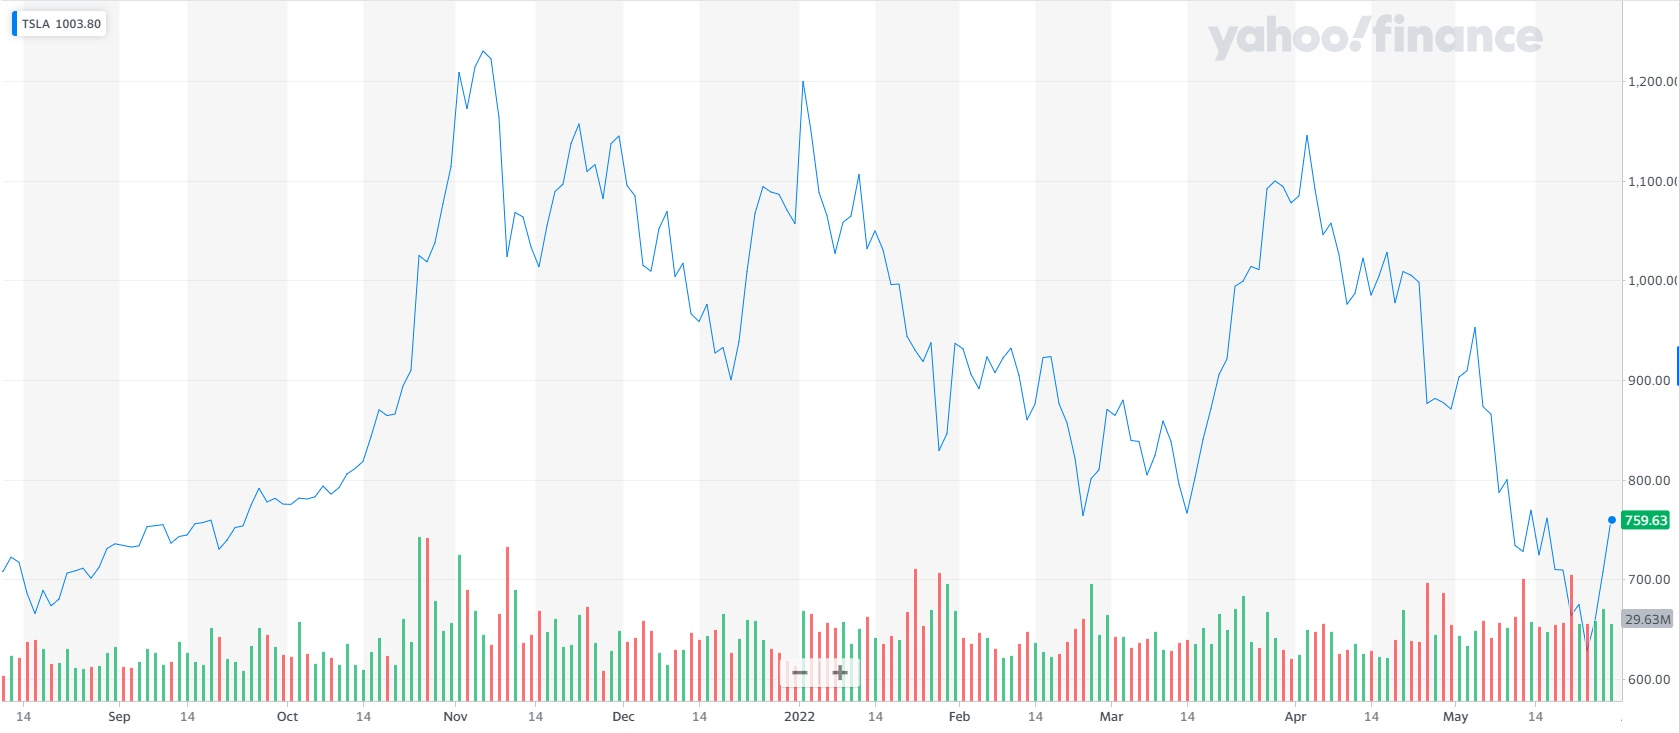
\includegraphics[width=0.8\textwidth]{pic/timeseries.jpg}
            \caption{Пример временного ряда}
        \end{figure}


        \subsection{Основы технического анализа}

            \subsubsection{Японская свеча}

            Графики свечей — наиболее популярная в Японии и самая древняя
            форма технического анализа. <<Японские свечи>> появились раньше, чем
            штриховые графики и графики «крестики-нолики». Японцы осознали важность 
            технического анализа давным-давно. Они первыми стали торговать
            фьючерсами. В середине XVII в. они торговали «пустыми» рисовыми 
            контрактами (рисом, которого еше не было, — иначе говоря, рисовыми 
            фьючерсами). [3]

            Японская свеча состоит из следующих компонентов: 
            \begin{enumerate}
                \item Open (цена открытия) "--- цена на начало периода.
                \item Close (цена закрытия) "--- цена на конец периода.
                \item High () "--- максимальная цена в течение периода.
                \item Close () "--- минимальная цена в течение периода.
            \end{enumerate}

            \begin{figure}[H]
                \centering
                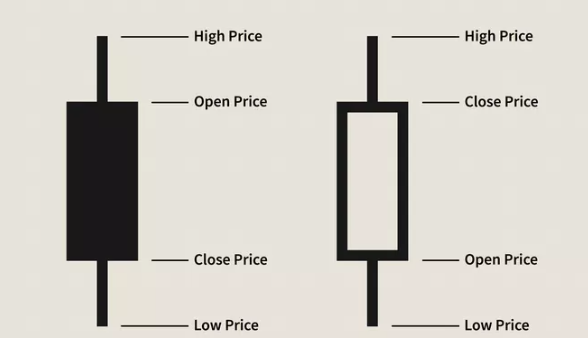
\includegraphics[width=0.8\textwidth]{pic/candlestick.png}
                \caption{Японская свеча}
            \end{figure}

            Для того, чтобы можно было отрисовать график акций, требуется использовать
            один из показателей японской свечи. В данной работе далее используется 
            показатель $Close$.

            \subsubsection{Определение тенденции с помощью макисмумов и минимумов}

                В качестве одного из стандартных методов определения тенденции
                повышения можно рассмотреть последовательности более высоких
                максимумов и более низких минимумов.    

                Итак, тенденция повышения является ненарушенной ровно до тех пор, 
                пока зафиксированный предыдущий относительный минимум не будет
                пробит, то есть не образуется новый минимум. Если такое происходит, 
                то делается вывод о том, что тенденция закончилась или же в 
                скором времени это произойдет.

                Аналогично можно определить и понижающую тенденцию как
                последовательность более низких минимумов и более низких максимумов.
                Понижающая тенденция является ненарушенной до тех пор, пока
                зафиксированный предыдущий максимум не пробит. Если же наблюдается
                пробитие максимума, то возможно понижающая тенденция подходит к
                своему завершению.

                \begin{figure}[H]
                    \centering
                    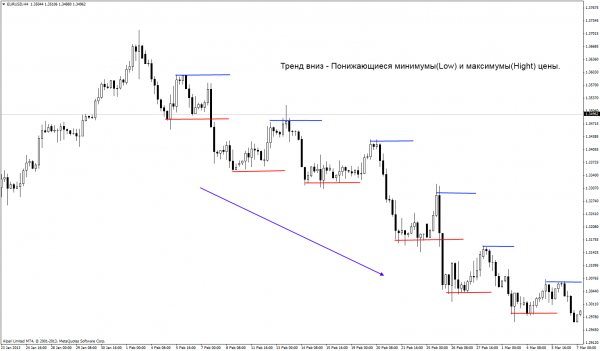
\includegraphics[width=0.8\textwidth]{pic/trand.png}
                    \caption{Пример нисходящего тренда}
                \end{figure}

            \subsubsection{Линия роста (падения)}
                Кумулятивная дневная линия роста / падения является одним из
                наиболее известных индикаторов разброса рынка и часто используется
                для обнаружения дивергенции (расхождения) с одним из свободных
                индексов рынка. Как правило, кумулятивная линия роста (падения) вычисляется как
                скользящая сумма чистого количества растущих акций.
                
                Вычисление значений линии роста (падения) проводится в два этапа:
                \begin{enumerate}
                    \item Вычисление разности между количеством растущих и количеством
                    падающих акций с сохранением знака результата. Полученное 
                    значение также называется \textit{чистым количеством растущих акций}.
                    \item Прибавить вычисленную сумму за данный день к значению
                    накопленной суммы ежедневных количеств \textit{растущих акций}.
                \end{enumerate}

                Также предлагается приступать к вычислению кумулятивной скользящей
                только после проведения нормализации дневных данных по формуле:
                \begin{center}
                    $N = \frac{A - D}{A + D} $, 
                \end{center}
                где $N$ "--- отношение чистого количества растущих акций к общему
                числу акций, показавших изменение цены, $A$ "--- количество растущих
                акций, $D$ "--- количество падающих акций.

        \subsection{Перцептрон как один из методов реализации нейронных сетей}
        
        Типичным примером модели глубокого обучения является глубокая сеть прямого 
        распространения, или многослойный перцептрон (МСП). Многослойный перцептрон 
        "--- это математическая функция, отображающая множество входных значений 
        на множество выходных. Эта функция является композицией нескольких
        более простых функций. Каждое применение одной математической функции можно
        рассматривать как новое представление входных данных.
        
        Глубина позволяет обучать многошаговую компьютерную программу. Каждый 
        слой представления можно мыслить себе как состояние памяти компьютера 
        после параллельного выполнения очередного набора инструкций. Чем больше 
        глубина сети, тем больше инструкций она может выполнить последовательно. 
        Последовательное выполнение инструкций расширяет возможности, поскольку 
        более поздние инструкции могут обращаться к результатам выполнения предыдущих.
        
        Есть два основных способа измерить глубину модели. Первый оценивает 
        архитектуру на основе числа последовательных инструкций, которые необходимо 
        выполнить. Можно считать, что это длина самого длинного пути в графе, 
        описывающем вычисление каждого выхода модели по ее входам. Как у двух 
        эквивалентных компьютерных программ могут быть разные длины пути в зависимости 
        от языка, на котором они написаны, так и одна и та же функциональность 
        может быть изображена графами с разной длиной пути в зависимости от того, 
        какие функции допускаются в качестве шагов. 

        При другом подходе, используемом в глубоких вероятностных моделях, глубиной
        модели считается не глубина графа вычислений, а глубина графа, описывающего
        связи концепций. В этом случае граф вычислений, выполняемых для вычисления
        представления каждой концепции, может быть гораздо глубже, чем граф самих 
        концепций. Связано это с тем, что понятие системы о простых концепциях можно 
        уточнять, располагая информацией о более сложных. Например, система ИИ, 
        наблюдающая изображение лица, на котором один глаз находится в тени, первоначально
        может распознать только один глаз. Но, обнаружив присутствие лица, система 
        может заключить, что должен быть и второй глаз. В таком случае граф концепций 
        содержит только два слоя – для глаз и для лиц, тогда как граф вычислений 
        содержит $2n$ слоев, если мы $n$ раз уточняем оценку каждой концепции при 
        известной информации о второй.

        Поскольку не всегда ясно, какой из двух подходов – глубина графа вычислений
        или глубина графа вероятностной модели – более релевантен, и поскольку разные 
        люди по-разному выбирают наборы примитивных элементов, из которых строятся
        графы, не существует единственно правильного значения глубины архитектуры, 
        как не существует единственно правильной длины компьютерной программы. И 
        нет общего мнения о том, какой должна быть глубина, чтобы модель можно было 
        считать <<глубокой>>. Однако можно все-таки сказать, что глубокое обучение 
        "--- это наука о моделях, в которых уровень композиции обученных функций 
        или обученных концепций выше, чем в традиционном машинном обучении.

        \subsection{Использование нейронных сетей для поиска фигур технического анализа}
        Существует целая теория распознавания изображений образов, являющаяся 
        разделом кибернетики.

        Нейронные сети в рассматриваемой задачи могут дать преимущество в связи 
        с тем, что они имеют афинную инвариантность к представляемым данным, в
        частности, к масштабу и углам смещения фигур технического анализа. Тогда
        данные отклонения можно считать шумом, с которым нейронная сеть, как
        правило умеет работать. 

        Одним из первых вопросов при использовании нейронной сети для нашей задачи
        является количество входов и подаваемая на них информация. Также важным 
        моментом является выбор типа нейронной сети, ее параметром и методов
        обучения. Рассматриваемая проблема относится к классу задач классификации, 
        а, значит, необходимо понять, к какой фигуре относится текущее поведение
        временного ряда.

        В качестве входной информации для нейронной сети можно использовать
        координаты начала отрезка, его окончания и угол наклона прямой. 

        Итак, для задачи о предсказании поведения текущего курса акций разумно
        в качестве нейросетевого ядра использовать многослойный перцептрон с
        обучением по методу обратного распространения ошибки. Данный тип нейронной
        сети хорошо зарекомендовал себя в задачах прогнозирования.

        На входы нейронной сети будут подаваться параметры нескольких подряд
        идущих отрезков. На выходе будут параметры следующего отрезка.
        
        Нейронные сети, безусловно, являются одним из методов поиска фигур
        технического анализа и предсказания поведения акций в зависимости от
        полученных результатов работы. В данной работе же рассматриваются 
        детерминированные подходы которые пытаются выделить технические фигуры
        на заданном временном ряде и затем провести прогнозирование поведения ряда
        в зависимости от найденных фигур.


\section{Практическая часть}

    \subsection{Описание инструментов и библиотек программной реализации}

        % Python
        В виду своей удобности использования, простоты написания кода, а также
        различных дополнительных библиотек для анализа акций, в данной работе 
        используется язык программирования Python. Простота применения Python для 
        написания кода и возможность его отладки через такие пакетные менеджеры, 
        как conda, упрощают обмен библиотеками и результатами исследований. 
        Его экосистема библиотек для работы в сфере трейдинга, таких как NumPy, 
        yfinance и Matplotlib, упрощают анализ результатов работы алгоритма, получение 
        котировок акций с различной временной градацией.
        % \cite{python}.

        %Yahoo Finance
        Yfinance "--- популярная библиотека с открытым исходным кодом, разработанная 
        Раном Арусси как средство доступа к финансовым данным, расположенным на
        ресурсе Yahoo Finance.

        Yahoo Finance предлагает обширный набор рыночных данных по акциям, 
        облигациям, валютам и криптовалютам. Для удобства использования в данной
        библиотеке присутствует возможность получения отчетов и анализов данных, 
        а также дополнительные параметры получаемых данных, что отличает его от 
        ряда конкурентов.

        Также стоит отметить, что отличительной особенностью yfinance является то, 
        что библиотека позволяет получить градуирование данных вплоть одной минуты. 
        Однако, что данные за текущий день получить нельзя. Если требуется 
        получить данные за день (то есть градуирование составляет по часам и меньше),
        то минимально возможная разница в днях с текущей датой составляет 60 дней.

        Получаемые данные представляют из себя $csv$-файл, в котором присутствуют
        вышеописанные элементы свечей: максимальная (минимальная) цена, открытие
        (закрытие) акции.

        %Matplotlib
        
        Matplotlib "--- это кроссплатформенная библиотека для визуализации данных 
        и графического построения графиков для Python и NumPy. В данной работе
        использование библиотеки является необходимым для отображения котировок
        акций и найденных фигур технического анализа с предполагаемым ростом (падением)
        курса. По оси абсцисс будем брать градуирование даты, а по оси ординат
        будем использовать полученные с помощью yfinance котировки, используя
        поле $close$.

        % \subsection{Описание набора данных}

        % Осуществление предобработки и принятие решения о выборе того или иного
        % набора данных для конкретной задачи машинного или глубокого обучения
        % является столь же важным этапом деятельности создания ИИ, как и
        % проектирование архитектуры модели и сопровождение процесса обучения.

        % В данной работе осуществляется решение задачи поиска технических фигур
        %   на акциях "--- следовательно, рациональнее и эффективнее
        % следует взять в качестве основного ресурса для обучения нейросети один
        % из таких наборов данных, как ''Microsoft COCO'', ''Visual Genome'',
        % ''TextCaps'', ''Flickr 8k'' и т.п. В качестве основополагающих данных
        % необязательно брать большой объем изображений с их текстовым описанием
        % "--- для проверки качества реализации нейросети достаточно выбрать
        % умеренное количество информации, и в связи с этим было принято решение
        % выбрать набор данных ''Flickr 8k'' (то есть исходя из других различных
        % исследовательских работ, связанных с генерацией текстового описания к
        % изображению) \cite{dataset1}, \cite{dataset2}.
        
        % Набор представляет собой эталонную коллекцию для генерации текстового
        % описания и поиска изображений на основе предложений на естественном
        % языке, которая состоит из более чем 8000 изображений, каждое из которых
        % имеет пять разных текстовых подписей, которые обеспечивают четкое
        % описание фигурирующих на конкретном изображении объектов и событий.
        % Изображения были выбраны из шести разных групп Flickr и, как правило, не
        % содержат каких-либо известных людей или мест, а были отобраны вручную
        % для отображения различных мероприятий и ситуаций. Набор данных находится
        % в открытом доступе и его можно загрузить как с официального сайта
        % фотохостинга, так и с других различных форумов и сайтов для машинного и
        % глубокого обучения \cite{dataset3}. В частности, для обучения модели,
        % описывающейся в данной работе, была взята такая коллекция совместно с
        % файлом формата CSV, в котором осуществляется сопоставление названия
        % каждого изображения с одним из его текстовых описаний.

        % Эти данные будут в дальнейшем поделены на тренировочную и тестовую
        % выборку, где первая выборка будет представлять собой 80\% от всего
        % набора данных, а тестовая "--- всё остальное.

        % \begin{figure}[H]
        %     \centering
        %     \includegraphics[width=1\textwidth]{pics/dataset.png}
        %     \caption{Содержимое CSV файла, в котором сопоставляется изображение
        %              с текстовым описанием}
        % \end{figure}

    %   \subsection{}
    % \subsection{Программная реализация алгоритма}

    %     Генератор подписей к входным изображениям будет представлять собой
    %     ансамбль из двух нейросетей - CNN и LSTM.

    %     Идея работы ансамбля заключается в том, что на вход к CNN подается
    %     цветное изображение (размеры которого предварительно сведены к 356
    %     пикселя в ширину и 356 пикселя в высоту). В качестве CNN будет
    %     использоваться модель GoogleNetv3, предобученная на датасете 2015-го
    %     года ImageNet.

\conclusion

    В данной работе были рассмотрены детерминированные методы поиска технических
    фигур на курсах акций. Проведен анализ работы алгоритма на акциях с высокой
    волатильностью и низкой, а также на акциях криптовалют. Алгоритм в некоторых
    случаях может работать некорректно в следствие неправильной подобранных
    значений допуска $eps$ в фигурах, где это значение используется. Также были 
    рассмотрены теоретические основы нейросетей, описаны основные
    принципы работы и их роль в решении, основы технического анализа и основные
    определения трейдинга. 

    В качестве практической части работы была описана программная реализация
    алгоритма поиска технических фигур на акциях, получение статистики по фигурам, 
    а также отрисовка данных фигур на графике акции с предполагаемым ростом или 
    падением курса.

\begin{thebibliography}{99}
    % https://secretmag.ru/enciklopediya/chto-takoe-volatilnost-obyasnyaem-prostymi-slovami.htm
    % https://www.investopedia.com/terms/t/timeseries.asp
    % https://www.investopedia.com/trading/candlestick-charting-what-is-it/
    % https://docs.google.com/file/d/0B7zVAgSBB3MeRXVVTmo2SzlfbFE/edit?resourcekey=0-cCN4jErXZGzi8bWmQU4bgA
    % https://finance.yahoo.com/
    % The encyclopedia of technical market indicators. Robert W. Colby
    % https://algotrading101.com/learn/yfinance-guide/ YAHOO FINANCE
    % https://www.activestate.com/resources/quick-reads/what-is-matplotlib-in-python-how-to-use-it-for-plotting/
    % https://scorum.ru/ru-ru/other/@goldenbogdan/fondovaya-birzha-v-1980-e-treiding-do-kompyuternoi-epokhi-kak-eto-bylo-chast-1

    % \bibitem{Gud} Гудфеллоу Я., Бенджио И., Курвилль А., ''Глубокое обучение'',
    % г. Москва, Издательство ДМК, 2018 г., Яз. рус.
    

    % \bibitem{neur} Короткий С., ''Нейронные сети: Основные положения'',
    % [Электронный ресурс] : [статья] / URL:
    % http://www.shestopaloff.ca/kyriako/Russian/Artificial_Intelligence/Some_publications/Korotky_Neuron_network_Lectures.pdf
    % (дата обращения 27.04.2022) Загл. с экрана. Яз. рус.
    
    % \bibitem{Gud} Гудфеллоу Я., Бенджио И., Курвилль А., ''Глубокое обучение'',
    % г. Москва, Издательство ДМК, 2018 г., Яз. рус.
    
    % % CNN
    % % https://arxiv.org/abs/1511.08458
    % % https://www.freecodecamp.org/news/an-intuitive-guide-to-convolutional-neural-networks-260c2de0a050/

    % \bibitem{cnn1} Keiron O'Shea, Ryan Nash, ''An Introduction to Convolutional
    % Neural Networks'', [Электронный ресурс] : [статья] / URL
    % https://arxiv.org/abs/1511.08458 (дата обращения 14.04.2022) Загл. с экрана.
    % Яз. англ.
    
    % \bibitem{cnn2} Daphne Cornelisse, ''An intuitive guide to Convolutional
    % Neural Networks'', [Электронный ресурс] : [статья] / URL
    % https://www.freecodecamp.org/news/an-intuitive-guide-to-convolutional-neural-networks-260c2de0a050/
    % (дата обращения 14.04.2022) Загл. с экрана. Яз. англ.

    % % RNN
    % % https://arxiv.org/pdf/1912.05911.pdf
    % % https://www.ibm.com/cloud/learn/recurrent-neural-networks
    
    % \bibitem{rnn1} Robin M. Schmidt, ''Recurrent Neural Networks (RNNs): A
    % gentle Introduction and Overview'', [Электронный ресурс] : [статья] / URL
    % https://arxiv.org/pdf/1912.05911.pdf (дата обращения 18.04.2022) Загл. с
    % экрана. Яз. англ.

    % \bibitem{rnn2} IBM Cloud Education, ''Recurrent Neural Networks'',
    % [Электронный ресурс] : [статья] / URL
    % https://www.ibm.com/cloud/learn/recurrent-neural-networks (дата обращения
    % 18.04.2022) Загл. с экрана. Яз. англ.

    % % LSTM
    % % https://arxiv.org/pdf/1909.09586.pdf
    % % https://habr.com/ru/company/wunderfund/blog/331310/

    % \bibitem{lstm1} Ralf C. Staudemeyer, Eric Rothstein Morris, ''Understanding
    % LSTM "--- a tutorial into Long Short-Term Memory Recurrent Neural Networks
    % '', [Электронный ресурс] : [статья] / URL
    % https://arxiv.org/pdf/1909.09586.pdf (дата обращения 22.04.2022) Загл. с
    % экрана. Яз. англ.

    % \bibitem{lstm2} Wunder Fund, ''LSTM – сети долгой краткосрочной памяти'',
    % [Электронный ресурс] : [статья] / URL
    % https://habr.com/ru/company/wunderfund/blog/331310/ (дата обращения
    % 22.04.2022) Загл. с экрана. Яз. рус.

    % % Metrics
    % % https://arxiv.org/ftp/arxiv/papers/1809/1809.03006.pdf
    % % https://arxiv.org/ftp/arxiv/papers/2006/2006.00887.pdf
    % % https://arxiv.org/pdf/1208.3145.pdf

    % \bibitem{metrics1} Alexei Botchkarev, ''Performance Metrics (Error Measures)
    % in Machine Learning Regression, Forecasting and Prognostics: Properties and
    % Typology'', [Электронный ресурс] : [статья] / URL
    % https://arxiv.org/ftp/arxiv/papers/1809/1809.03006.pdf (дата обращения
    % 24.04.2022) Загл. с экрана. Яз. англ.

    % \bibitem{metrics2} M.Z. Naser, Amir H. Alavi, ''Insights into Performance
    % Fitness and Error Metrics for Machine Learning'', [Электронный ресурс] :
    % [статья] / URL https://arxiv.org/ftp/arxiv/papers/2006/2006.00887.pdf (дата
    % обращения 24.04.2022) Загл. с экрана. Яз. англ.

    % \bibitem{metrics3} Stijn Van dongen, Anton J. Enright, ''METRIC DISTANCES
    % DERIVED FROM COSINE SIMILARITY AND PEARSON AND SPEARMAN CORRELATIONS'',
    % [Электронный ресурс] : [статья] / URL https://arxiv.org/pdf/1208.3145.pdf
    % (дата обращения 24.04.2022) Загл. с экрана. Яз. англ.

    % % Cross Entropy Loss
    % % https://arxiv.org/pdf/2011.05231.pdf
    % % https://arxiv.org/pdf/2006.14822.pdf

    % \bibitem{celoss1} Elliott Gordon-Rodriguez, Gabriel Loaiza-Ganem и т.д.,
    % ''Uses and Abuses of the Cross-Entropy Loss: Case Studies in Modern Deep
    % Learning'', [Электронный ресурс] : [статья] / URL
    % https://arxiv.org/pdf/2011.05231.pdf (дата обращения 27.04.2022) Загл. с
    % экрана. Яз. англ.

    % \bibitem{celoss2} Shruti Jadon, ''A survey of loss functions for semantic
    % segmentation'', [Электронный ресурс] : [статья] / URL
    % https://arxiv.org/pdf/2006.14822.pdf (дата обращения 27.04.2022) Загл. с
    % экрана. Яз. англ.

    % % Relu
    % % https://arxiv.org/pdf/1803.08375.pdf
    % % https://arxiv.org/pdf/2107.09370.pdf

    % \bibitem{relu1} Abien Fred M. Agarap, ''Deep Learning using Rectified Linear
    % Units (ReLU)'', [Электронный ресурс] : [статья] / URL
    % https://arxiv.org/pdf/1803.08375.pdf (дата обращения 28.04.2022) Загл. с
    % экрана. Яз. англ.

    % \bibitem{relu2} Pierre Stock, Remi Gribonval, ''AN EMBEDDING OF RELU
    % NETWORKS AND AN ANALYSIS OF THEIR IDENTIFIABILITY'', [Электронный ресурс] :
    % [статья] / URL https://arxiv.org/pdf/2107.09370.pdf (дата обращения
    % 28.04.2022) Загл. с экрана. Яз. англ.
    

    % % https://mobidev.biz/blog/exploring-deep-learning-image-captioning
    % \bibitem{applications} Diana Malyk, ''Exploring Deep Learning Image
    % Captioning'', [Электронный ресурс] : [статья] / URL
    % https://mobidev.biz/blog/exploring-deep-learning-image-captioning (дата
    % обращения 30.04.2022) Загл. с экрана. Яз. англ.

    % % Python
    % % https://arxiv.org/pdf/2104.00254.pdf
    % \bibitem{python} Zachary DeVito, Jason Ansel и т.д., ''USING PYTHON FOR MODEL
    % INFERENCE IN DEEP LEARNING'', [Электронный ресурс] : [статья] / URL
    % https://arxiv.org/pdf/2104.00254.pdf (дата обращения 2.05.2022) Загл. с
    % экрана. Яз. англ.
    % % PIL
    % % https://pypi.org/project/Pillow/
    % \bibitem{pil} Alex Clark и т.д., ''Pillow'', [Электронный ресурс] : [статья]
    % / URL https://pillow.readthedocs.io/en/stable/ (дата обращения 2.05.2022)
    % Загл. с экрана. Яз. англ.
    % % Pandas
    % % https://vk.com/doc44301783_570833604?hash=LGYlshZgzLYwudBTZs1qE7XYb8l9puWt8uHniCTh6Zs&dl=icFVk5kLe613AvNLwIwLfFlkaiWT6odCWzRf3ZMgQXL
    % \bibitem{pandas} Маккинни У., ''Python и анализ данных'', ДМК Пресс, 2015.
    % "--- 482 с. "--- ISBN 978-5-97060-315-4, 978-1-449-31979-3.
    % % Spacy
    % % https://arxiv.org/pdf/2106.07799.pdf
    % \bibitem{spacy} Hannah Eyre, Alec B Chapman и т.д., ''Launching into clinical
    % space with medspaCy: a new clinical text processing toolkit in Python'',
    % [Электронный ресурс] : [статья] / URL https://arxiv.org/pdf/2106.07799.pdf
    % (дата обращения 2.05.2022) Загл. с экрана. Яз. англ.
    % % PyTorch
    % \bibitem{pytorch} Adam Paszke, Sam Gross и т.д., ''PyTorch: An Imperative
    % Style, High-Performance Deep Learning Library'', [Электронный ресурс] :
    % [статья] / URL https://arxiv.org/pdf/1912.01703.pdf (дата обращения
    % 2.05.2022) Загл. с экрана. Яз. англ.
    % % Torchvision

    % % Dataset
    % \bibitem{dataset1} Vikram Mullachery, Vishal Motwani, ''Image Captioning'',
    % [Электронный ресурс] : [статья] / URL https://arxiv.org/pdf/1805.09137.pdf
    % (дата обращения 8.05.2022) Загл. с экрана. Яз. англ.

    % \bibitem{dataset2} Kelvin Xu, Jimmy Lei Ba и т.д., ''Show, Attend and
    % Tell: Neural Image Caption Generation with Visual Attention'', [Электронный
    % ресурс] : [статья] / URL https://arxiv.org/pdf/1502.03044.pdf (дата
    % обращения 8.05.2022) Загл. с экрана. Яз. англ.

    % \bibitem{dataset3} ADITYAJN105, ''Flickr 8k Dataset '', [Электронный ресурс]
    % : [статья] / URL https://www.kaggle.com/datasets/adityajn105/flickr8k (дата
    % обращения 8.05.2022) Загл. с экрана. Яз. англ.

    % % model

    % \bibitem{inception} Pytorch Team, ''INCEPTION_V3'', [Электронный ресурс] :
    % [статья] / URL https://pytorch.org/hub/pytorch_vision_inception_v3/ (дата
    % обращения 8.05.2022) Загл. с экрана. Яз. англ.

    % % hyperparams

    % \bibitem{embedding} Adam Schwab, ''Embeddings: A Matrix of Meaning'',
    % [Электронный ресурс] : [статья] / URL
    % https://petuum.medium.com/embeddings-a-matrix-of-meaning-4de877c9aa27 (дата
    % обращения 8.05.2022) Загл. с экрана. Яз. англ.

    \bibitem{learningrate} Zelun Luo, Boya Peng и т.д., ''Show, Discriminate,
    and Tell: A Discriminatory Image Captioning Model with Deep Neural
    Networks'', [Электронный ресурс] : [статья] / URL
    https://web.stanford.edu/class/cs231a/prev_projects_2016/cs231a.pdf (дата
    обращения 8.05.2022) Загл. с экрана. Яз. англ.

    % results
    
    \bibitem{fitting} Ritter F. E., Schooler L. J., ''The learning curve'',
    [Электронный ресурс] : [статья] / URL
    http://ritter.ist.psu.edu/papers/ritterS01.pdf (дата обращения 12.05.2022)
    Загл. с экрана. Яз. англ.


\end{thebibliography}

\appendix

    \section{Код drawing.py}
    \inputminted[fontsize=\footnotesize]{text}{code/drawing.py}

    \section{Код figures.py}
    \inputminted[fontsize=\footnotesize]{text}{code/figures.py}

    \section{Код main.py}
    \inputminted[fontsize=\footnotesize]{text}{code/main.py}

\end{document}
